
\subsubsection{Reconstruction of $Q^2$ and $x$}\label{sec:ana_q2}

The four-momentum transfer squared is 
\begin{equation} \label{eq:qsq}
Q^2 \hskip 0.05in
= \hskip 0.05in 2 \hskip 0.02in E \hskip 0.02in 
E^{\prime} \hskip 0.02in (1- {\rm cos}(\theta))
\end{equation}
where $E$ is the incident energy, $E^{\prime}$ is the
final momentum or energy of the 
electron ($E^{\prime} \gg m_e$) and
$\theta$ is the scattering angle.  

For the beam energy we used the Tiefenbach energy (need to 
explain this) of ??? GeV
and assumed a 3 MeV (???) average energy loss to the center of the 
target which is applied
this as a correction to the beam energy.  
The error in the beam energy $E$ and $E^{\prime}$ are assumed
conservatively to be 3 MeV based on a history of these measurements
in Hall A.  The most important error is in $\theta$ ...

Perhaps need a table of errors.

%the following is copied from Bob's v1 but according to the new outline should be separated into two simulations. The HAMC should go into section ``Q2 reconstruction'' (above), the HATS should be a stand-alone subsection of ``Analysis''.

\subsection{Simulation}

Two simulation packages were used to support the analysis of this experiment.
The package called ``hamc'' (Hall A Monte Carlo) was used to simulate
the events and the spectrometer acceptance, while a second package
called ``hats'' (Hall A Trigger Simulation) was used to simulate the
response of the trigger used to identify electrons and pions, providing
a calculation of our deadtime.

In ``hamc'', events are generated using a physics class that has information about the cross section and asymmetry.  
The tracks are generated uniformly in solid angle 
\hskip 0.05in $d\Omega = sin(\theta) \hskip 0.02in d\theta \hskip 0.02in d\phi$ \hskip 0.05in and 
the results later weighted by the differential cross section $\frac{d\sigma}{d\Omega}$. 
The simulated tracks undergo multiple scattering in the target and 
energy loss from the target from external and internal Brehmstrahlung as 
well as ionization loss, 

The generated four-vectors are transported to the detector in the HRS focal plane using 
a set of polynomials that model the trajectories of electrons through the magnetic fields.
The beam raster is simulated, which produces a smearing of the beam on target.
The events are transported to intermediate apertures such as the collimator 
or the entrance to quadrupoles. 
Events that reach the HRS focal plane and intersect the detectors are integrated 
to compute the total rate and average asymmetry.

The acceptance of the HRS is generally defined by combining the openning geometry of the intermediate apertures, the norminal settings of which is documented in [Hall A NIM]. In real experiment, however, the edge of the opennings are not well defined, as events falling on the edge may correspond to electrons scattering from the aperture's material. Therefore, the real acceptance can be different from the norminal settings.We furtherly fine-tune the HRS acceptance of the simulation in the following way: taking the target variables of good events from data as the starting point, we use the same transport function as in HAMC to transport these data four-vectors to different apertures, and then read off the edges of the data patern as the real geometry to define the acceptance. This process is illustrated in Fig.~\ref{fig:hamc_acc}.

\begin{figure}[!pt]
\centering
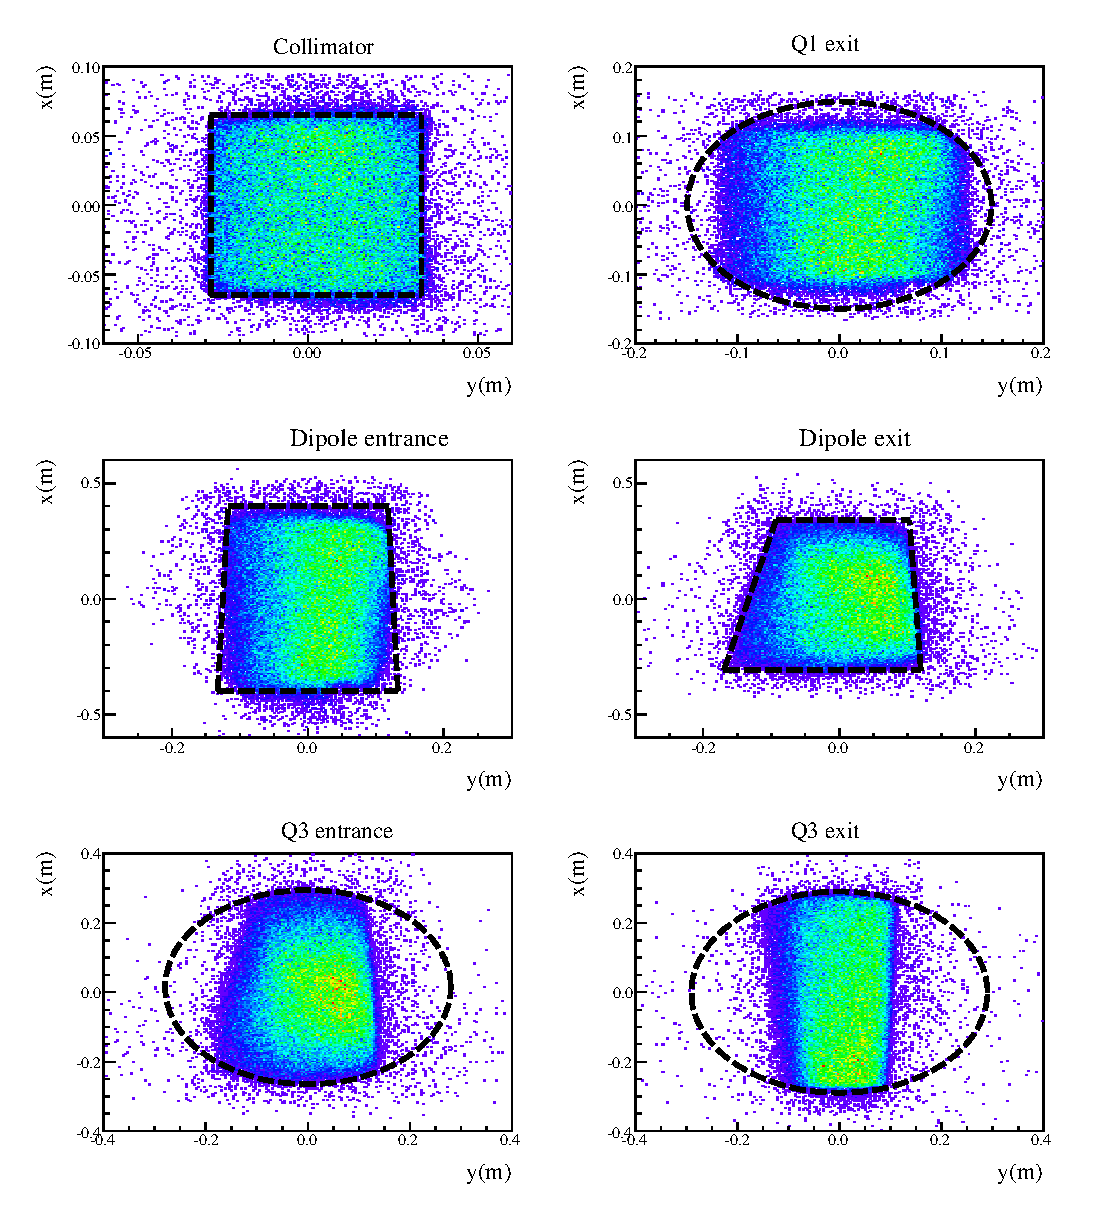
\includegraphics{DW/acceptance.eps}
\caption{HAMC acceptance tuning. Plotted are the $x$ and $y$ cordinates of data events transported to different apertures. Black lines are the geometry shapes determined according to the data plots, which will be used as acceptance cuts in HAMC.}\label{fig:hamc_acc}
\end{figure}

\begin{figure}[!p]
\centering
\includegraphics{DW/compl_tg.eps}
\includegraphics{DW/compl_Qx.eps}
\caption{Comparison between HAMC and data for Left HRS kinematics \#1.}\label{fig:hamc_compl}
\end{figure}

\begin{figure}[!p]
\centering
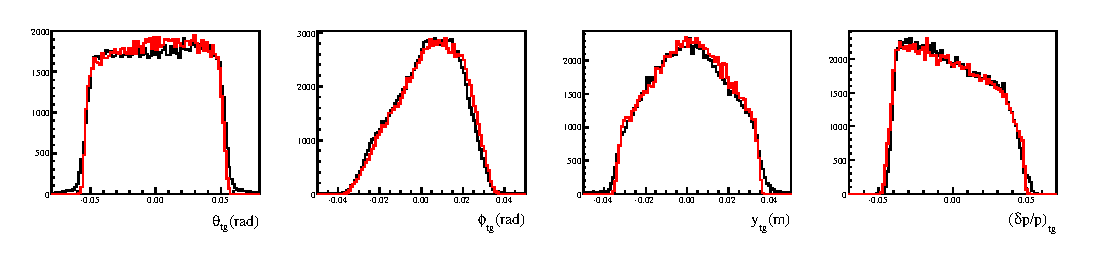
\includegraphics{DW/compr_tg.eps}
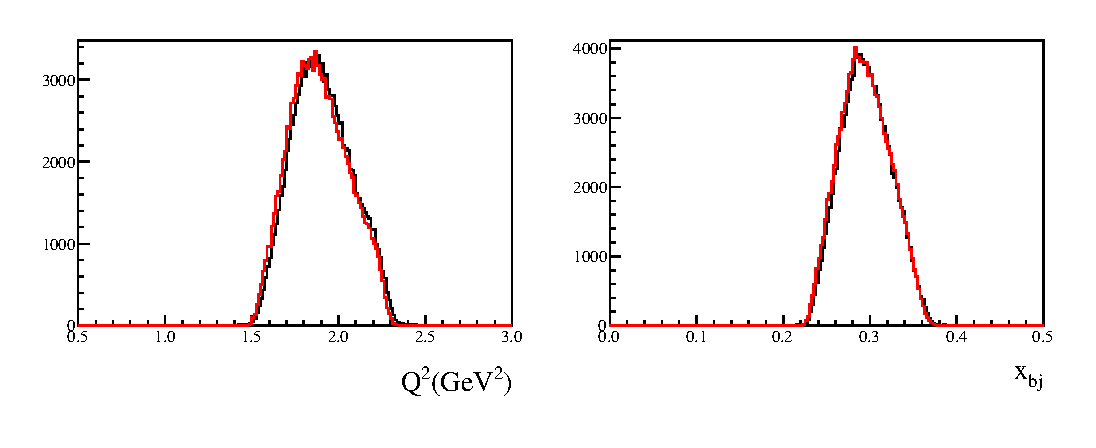
\includegraphics{DW/compr_Qx.eps}
\caption{Comparison between HAMC and data for Right HRS kinematics \#2.}\label{fig:hamc_compr}
\end{figure}

The quality of ``hamc'' is checked by the comparison between simulation results and data on the target variables and kinematics variables. Fig.~\ref{fig:hamc_compl} (Fig.~\ref{fig:hamc_compr}) show such comparisons for Left (Right) HRS. The simulation agrees well with data. 

Here describe ``hats'' ...

